% !TEX program = xelatex
\documentclass[a4paper,10pt]{article}
\usepackage[margin=2.05cm]{geometry}
\usepackage{fontspec}
\usepackage{graphicx}
\usepackage{booktabs}
\usepackage{longtable}
\usepackage{tabularx}
\usepackage{array}
\usepackage{amsmath}
\usepackage{microtype}
\usepackage{xcolor}
\usepackage{hyperref}
\usepackage{caption}
\usepackage{float}
\usepackage[section]{placeins}
\usepackage[numbers,sort&compress]{natbib}
\graphicspath{{figures/}}
% Generated by scripts/generate_dataset_figures.py.
\newcommand{\DatasetSceneCount}{10}
\newcommand{\DatasetTiffCount}{60}
\newcommand{\DatasetUsablePatchCount}{1800}
\newcommand{\DatasetPrivacyExcludedCount}{25}
\newcommand{\DatasetFixedTrainCount}{1141}
\newcommand{\DatasetFixedValidationCount}{270}
\newcommand{\DatasetFixedTestCount}{389}
\newcommand{\DatasetTaskFileCount}{14400}
\newcommand{\DatasetRawFileCount}{1281}
\newcommand{\DatasetSourcePositionCount}{140}
\newcommand{\DatasetRgbFrameCount}{581}
\newcommand{\DatasetSwirFrameCount}{700}
\newcommand{\DatasetPoseEdgeCount}{591}
\newcommand{\DatasetOutputScale}{3.2}
\newcommand{\DatasetAcquisitionDateMin}{2025-04-29}
\newcommand{\DatasetAcquisitionDateMax}{2025-11-28}
\newcommand{\DatasetCoverageMin}{0.712}
\newcommand{\DatasetCoverageMax}{0.902}
\newcommand{\DatasetCoverageMean}{0.841}
\newcommand{\DatasetBuildSecondsMin}{48.6}
\newcommand{\DatasetBuildSecondsMax}{908.1}
\newcommand{\DatasetRedactedSceneUsablePatchCount}{131}
\newcommand{\RegHoldoutMinPx}{3.56}
\newcommand{\RegHoldoutMedianPx}{5.73}
\newcommand{\RegHoldoutMeanPx}{6.06}
\newcommand{\RegHoldoutMaxPx}{9.23}
\newcommand{\RegCornerMinPx}{1.56}
\newcommand{\RegCornerMedianPx}{3.03}
\newcommand{\RegCornerMeanPx}{5.70}
\newcommand{\RegCornerMaxPx}{27.78}
\newcommand{\RegCornerWorstScene}{C5}
\newcommand{\RegCornerRunnerUpPx}{8.60}
\newcommand{\RegCornerOutlierRatio}{3.2}
\newcommand{\RegCornerOtherMeanPx}{3.24}
\newcommand{\RegCornerGateMinPx}{25.6}
\newcommand{\RegCornerGateMaxPx}{76.3}
\newcommand{\IntraSwirMinPx}{3.19}
\newcommand{\IntraSwirMeanPx}{4.74}
\newcommand{\IntraSwirMaxPx}{6.25}
\newcommand{\IntraSwirGatePx}{8}

% Generated by scripts/build_geom_diagnostics.py; do not edit manually.
\newcommand{\GeomRgbBOnePrevMin}{0.77}
\newcommand{\GeomRgbBOnePrevMax}{1.92}
\newcommand{\GeomRgbBOneOutMin}{3.56}
\newcommand{\GeomRgbBOneOutMax}{12.97}
\newcommand{\GeomCornerPrevMin}{0.28}
\newcommand{\GeomCornerPrevMax}{1.72}
\newcommand{\GeomIntraSwirMin}{3.48}
\newcommand{\GeomIntraSwirMax}{6.25}
\newcommand{\GeomBaBeforeMin}{0.42}
\newcommand{\GeomBaBeforeMax}{2.26}
\newcommand{\GeomBaAfterMin}{0.41}
\newcommand{\GeomBaAfterMax}{0.84}
\newcommand{\GeomBaHoldoutMin}{1.06}
\newcommand{\GeomBaHoldoutMax}{2.08}
\newcommand{\GeomCovMin}{71.2}
\newcommand{\GeomCovMax}{89.2}

\newcommand{\AuditTotalTiles}{432}
\newcommand{\AuditTotalChecks}{6480}
\newcommand{\AuditJudgeablePct}{71.3}
\newcommand{\AuditRgbSwirMed}{2.37}
\newcommand{\AuditRgbSwirRmse}{3.85}
\newcommand{\AuditRgbSwirPnineFive}{7.97}
\newcommand{\AuditRgbSwirJudPct}{49.8}
\newcommand{\AuditSwirSwirMed}{0.51}
\newcommand{\AuditSwirSwirRmse}{1.73}
\newcommand{\AuditSwirSwirPnineFive}{2.84}
\newcommand{\AuditSwirSwirJudPct}{82.0}
\newcommand{\AuditRgbHiMed}{2.20}
\newcommand{\AuditRgbLoMed}{2.68}
\newcommand{\AuditSwirHiMed}{0.50}
\newcommand{\AuditSwirLoMed}{0.54}

\newcommand{\TrackCDrZsPsnr}{13.378}
\newcommand{\TrackCDrZsDe}{23.505}
\newcommand{\TrackCDrScPsnr}{14.458}
\newcommand{\TrackCDrScDe}{17.728}
\newcommand{\TrackCDrFtPsnr}{14.448}
\newcommand{\TrackCDrFtDe}{17.808}
\newcommand{\TrackCDrFtGainZs}{+1.070}
\newcommand{\TrackCDrFtGainQuad}{-2.267}

% Generated from bundled saved records; do not edit.
\newcommand{\SupportPixelCount}{88861466}
\newcommand{\QualifiedWindowCount}{5893}
\newcommand{\LpipsRectCount}{1541}
\newcommand{\FormalRunCount}{225}
\newcommand{\RandomRunCount}{45}
\newcommand{\ProtocolGain}{4.435}
\newcommand{\CalibrationAffineGain}{2.389}
\newcommand{\CalibrationQuadIncrement}{0.213}
\newcommand{\CalibrationCross}{14.113}
\newcommand{\CalibrationTarget}{16.502}
\newcommand{\CalibrationQuad}{16.715}
\newcommand{\HalfWithin}{17.432}
\newcommand{\HalfCross}{15.587}
\newcommand{\HalfDrop}{1.845}
\newcommand{\DrunetGain}{0.202}
\newcommand{\DrunetSingle}{13.619}
\newcommand{\DrunetTriple}{13.820}
\newcommand{\PixGain}{-0.020}
\newcommand{\PixSingle}{12.876}
\newcommand{\PixTriple}{12.856}
\newcommand{\TfdGain}{0.800}
\newcommand{\TfdSingle}{12.040}
\newcommand{\TfdTriple}{12.839}

\newcommand{\MsEpHundredPsnr}{24.46}
\newcommand{\MsEpHundredPsnrSd}{1.12}
\newcommand{\MsEpHundredPsnrPm}{24.46$\pm$1.12}
\newcommand{\MsEpHundredSsim}{0.807}
\newcommand{\MsEpHundredSsimSd}{0.011}
\newcommand{\MsEpHundredSsimPm}{0.807$\pm$0.011}
\newcommand{\MsEpHundredLpips}{0.089}
\newcommand{\MsEpHundredLpipsSd}{0.029}
\newcommand{\MsEpHundredLpipsPm}{0.089$\pm$0.029}
\newcommand{\MsEpTwoHundredPsnr}{28.88}
\newcommand{\MsEpTwoHundredPsnrSd}{0.06}
\newcommand{\MsEpTwoHundredPsnrPm}{28.88$\pm$0.06}
\newcommand{\MsEpTwoHundredSsim}{0.871}
\newcommand{\MsEpTwoHundredSsimSd}{0.000}
\newcommand{\MsEpTwoHundredSsimPm}{0.871$\pm$0.000}
\newcommand{\MsEpTwoHundredLpips}{0.033}
\newcommand{\MsEpTwoHundredLpipsSd}{0.000}
\newcommand{\MsEpTwoHundredLpipsPm}{0.033$\pm$0.000}
\newcommand{\ChEpHundredPsnr}{20.26}
\newcommand{\ChEpHundredPsnrSd}{1.80}
\newcommand{\ChEpHundredPsnrPm}{20.26$\pm$1.80}
\newcommand{\ChEpHundredSsim}{0.674}
\newcommand{\ChEpHundredSsimSd}{0.040}
\newcommand{\ChEpHundredSsimPm}{0.674$\pm$0.040}
\newcommand{\ChEpHundredLpips}{0.136}
\newcommand{\ChEpHundredLpipsSd}{0.057}
\newcommand{\ChEpHundredLpipsPm}{0.136$\pm$0.057}
\newcommand{\ChEpTwoHundredPsnr}{22.91}
\newcommand{\ChEpTwoHundredPsnrSd}{0.18}
\newcommand{\ChEpTwoHundredPsnrPm}{22.91$\pm$0.18}
\newcommand{\ChEpTwoHundredSsim}{0.741}
\newcommand{\ChEpTwoHundredSsimSd}{0.006}
\newcommand{\ChEpTwoHundredSsimPm}{0.741$\pm$0.006}
\newcommand{\ChEpTwoHundredLpips}{0.074}
\newcommand{\ChEpTwoHundredLpipsSd}{0.002}
\newcommand{\ChEpTwoHundredLpipsPm}{0.074$\pm$0.002}
\newcommand{\NativeEpHundredPsnr}{18.02}
\newcommand{\NativeEpHundredPsnrSd}{--}
\newcommand{\NativeEpHundredPsnrPm}{18.02}
\newcommand{\NativeEpHundredSsim}{0.551}
\newcommand{\NativeEpHundredSsimSd}{--}
\newcommand{\NativeEpHundredSsimPm}{0.551}
\newcommand{\NativeEpHundredLpips}{0.404}
\newcommand{\NativeEpHundredLpipsSd}{--}
\newcommand{\NativeEpHundredLpipsPm}{0.404}
\newcommand{\NativeEpTwoHundredPsnr}{20.72}
\newcommand{\NativeEpTwoHundredPsnrSd}{--}
\newcommand{\NativeEpTwoHundredPsnrPm}{20.72}
\newcommand{\NativeEpTwoHundredSsim}{0.577}
\newcommand{\NativeEpTwoHundredSsimSd}{--}
\newcommand{\NativeEpTwoHundredSsimPm}{0.577}
\newcommand{\NativeEpTwoHundredLpips}{0.283}
\newcommand{\NativeEpTwoHundredLpipsSd}{--}
\newcommand{\NativeEpTwoHundredLpipsPm}{0.283}
\newcommand{\MsEpFiveHundredPsnr}{30.18}
\newcommand{\MsEpFiveHundredPsnrSd}{--}
\newcommand{\MsEpFiveHundredPsnrPm}{30.18}
\newcommand{\MsEpFiveHundredSsim}{0.905}
\newcommand{\MsEpFiveHundredSsimSd}{--}
\newcommand{\MsEpFiveHundredSsimPm}{0.905}
\newcommand{\MsEpFiveHundredLpips}{0.025}
\newcommand{\MsEpFiveHundredLpipsSd}{--}
\newcommand{\MsEpFiveHundredLpipsPm}{0.025}
\newcommand{\ChEpFiveHundredPsnr}{23.25}
\newcommand{\ChEpFiveHundredPsnrSd}{0.59}
\newcommand{\ChEpFiveHundredPsnrPm}{23.25$\pm$0.59}
\newcommand{\ChEpFiveHundredSsim}{0.774}
\newcommand{\ChEpFiveHundredSsimSd}{0.004}
\newcommand{\ChEpFiveHundredSsimPm}{0.774$\pm$0.004}
\newcommand{\ChEpFiveHundredLpips}{0.079}
\newcommand{\ChEpFiveHundredLpipsSd}{0.017}
\newcommand{\ChEpFiveHundredLpipsPm}{0.079$\pm$0.017}
\newcommand{\FracTwentyFivePsnr}{24.15}
\newcommand{\FracTwentyFivePsnrSd}{--}
\newcommand{\FracTwentyFivePsnrPm}{24.15}
\newcommand{\FracTwentyFiveSsim}{0.794}
\newcommand{\FracTwentyFiveSsimSd}{--}
\newcommand{\FracTwentyFiveSsimPm}{0.794}
\newcommand{\FracTwentyFiveLpips}{0.085}
\newcommand{\FracTwentyFiveLpipsSd}{--}
\newcommand{\FracTwentyFiveLpipsPm}{0.085}
\newcommand{\FracFiftyPsnr}{24.68}
\newcommand{\FracFiftyPsnrSd}{--}
\newcommand{\FracFiftyPsnrPm}{24.68}
\newcommand{\FracFiftySsim}{0.806}
\newcommand{\FracFiftySsimSd}{--}
\newcommand{\FracFiftySsimPm}{0.806}
\newcommand{\FracFiftyLpips}{0.071}
\newcommand{\FracFiftyLpipsSd}{--}
\newcommand{\FracFiftyLpipsPm}{0.071}
\newcommand{\FracSeventyFivePsnr}{24.06}
\newcommand{\FracSeventyFivePsnrSd}{--}
\newcommand{\FracSeventyFivePsnrPm}{24.06}
\newcommand{\FracSeventyFiveSsim}{0.803}
\newcommand{\FracSeventyFiveSsimSd}{--}
\newcommand{\FracSeventyFiveSsimPm}{0.803}
\newcommand{\FracSeventyFiveLpips}{0.096}
\newcommand{\FracSeventyFiveLpipsSd}{--}
\newcommand{\FracSeventyFiveLpipsPm}{0.096}
\newcommand{\FracTwentyFiveEpHundredPsnr}{21.79}
\newcommand{\FracTwentyFiveEpHundredPsnrSd}{--}
\newcommand{\FracTwentyFiveEpHundredPsnrPm}{21.79}
\newcommand{\FracTwentyFiveEpHundredSsim}{0.695}
\newcommand{\FracTwentyFiveEpHundredSsimSd}{--}
\newcommand{\FracTwentyFiveEpHundredSsimPm}{0.695}
\newcommand{\FracTwentyFiveEpHundredLpips}{0.125}
\newcommand{\FracTwentyFiveEpHundredLpipsSd}{--}
\newcommand{\FracTwentyFiveEpHundredLpipsPm}{0.125}
\newcommand{\FracFiftyEpHundredPsnr}{23.71}
\newcommand{\FracFiftyEpHundredPsnrSd}{--}
\newcommand{\FracFiftyEpHundredPsnrPm}{23.71}
\newcommand{\FracFiftyEpHundredSsim}{0.760}
\newcommand{\FracFiftyEpHundredSsimSd}{--}
\newcommand{\FracFiftyEpHundredSsimPm}{0.760}
\newcommand{\FracFiftyEpHundredLpips}{0.089}
\newcommand{\FracFiftyEpHundredLpipsSd}{--}
\newcommand{\FracFiftyEpHundredLpipsPm}{0.089}
\newcommand{\FracSeventyFiveEpHundredPsnr}{24.28}
\newcommand{\FracSeventyFiveEpHundredPsnrSd}{--}
\newcommand{\FracSeventyFiveEpHundredPsnrPm}{24.28}
\newcommand{\FracSeventyFiveEpHundredSsim}{0.788}
\newcommand{\FracSeventyFiveEpHundredSsimSd}{--}
\newcommand{\FracSeventyFiveEpHundredSsimPm}{0.788}
\newcommand{\FracSeventyFiveEpHundredLpips}{0.087}
\newcommand{\FracSeventyFiveEpHundredLpipsSd}{--}
\newcommand{\FracSeventyFiveEpHundredLpipsPm}{0.087}
\newcommand{\SceneFoldAPsnr}{7.64}
\newcommand{\SceneFoldAPsnrSd}{--}
\newcommand{\SceneFoldAPsnrPm}{7.64}
\newcommand{\SceneFoldASsim}{0.186}
\newcommand{\SceneFoldASsimSd}{--}
\newcommand{\SceneFoldASsimPm}{0.186}
\newcommand{\SceneFoldALpips}{0.764}
\newcommand{\SceneFoldALpipsSd}{--}
\newcommand{\SceneFoldALpipsPm}{0.764}
\newcommand{\SceneFoldBPsnr}{7.84}
\newcommand{\SceneFoldBPsnrSd}{--}
\newcommand{\SceneFoldBPsnrPm}{7.84}
\newcommand{\SceneFoldBSsim}{0.164}
\newcommand{\SceneFoldBSsimSd}{--}
\newcommand{\SceneFoldBSsimPm}{0.164}
\newcommand{\SceneFoldBLpips}{0.696}
\newcommand{\SceneFoldBLpipsSd}{--}
\newcommand{\SceneFoldBLpipsPm}{0.696}
\newcommand{\MsEpHundredSeeds}{3}
\newcommand{\MsEpTwoHundredSeeds}{3}
\newcommand{\ChEpHundredSeeds}{3}
\newcommand{\ChEpTwoHundredSeeds}{3}
\newcommand{\MsEpHundredRunMin}{23.17}
\newcommand{\MsEpHundredRunMax}{25.22}
\newcommand{\MsEpHundredRunSpan}{2.06}
\newcommand{\MsEpTwoHundredRunMin}{28.81}
\newcommand{\MsEpTwoHundredRunMax}{28.93}
\newcommand{\MsEpTwoHundredRunSpan}{0.12}
\newcommand{\ChEpHundredRunMin}{18.18}
\newcommand{\ChEpHundredRunMax}{21.33}
\newcommand{\ChEpHundredRunSpan}{3.14}
\newcommand{\ChEpTwoHundredRunMin}{22.76}
\newcommand{\ChEpTwoHundredRunMax}{23.10}
\newcommand{\ChEpTwoHundredRunSpan}{0.35}
\newcommand{\MsEpHundredLowRunGap}{2.06}
\newcommand{\MsEpTwoHundredLowRunGap}{0.03}
\newcommand{\ChEpHundredLowRunGap}{3.14}
\newcommand{\ChEpTwoHundredLowRunGap}{0.23}
\newcommand{\NativeDropHundred}{6.44}
\newcommand{\NativeDropTwoHundred}{8.16}
\newcommand{\ChLateSwing}{0.84}
\newcommand{\GapEpHundred}{+4.19}
\newcommand{\GapEpTwoHundred}{+5.97}
\newcommand{\GapEpHundredPlain}{4.19}
\newcommand{\GapEpTwoHundredPlain}{5.97}
\newcommand{\BudgetGainTwentyFive}{+0.31}
\newcommand{\BudgetGainFifty}{-0.22}
\newcommand{\BudgetGainSeventyFive}{+0.39}
\newcommand{\SceneHeldEqualPsnr}{8.58}
\newcommand{\SceneRandomEqualPsnr}{24.27}
\newcommand{\SceneDropEqualAbs}{15.68}
\newcommand{\SceneDropEqualPsnr}{+15.68}
\newcommand{\SceneDropFoldPsnr}{+16.72}
\newcommand{\SceneHeldLowerCount}{10}
\newcommand{\SceneHeldSceneCount}{10}
\newcommand{\SceneHeldMinName}{C1}
\newcommand{\SceneHeldMinPsnr}{5.13}
\newcommand{\SceneHeldMaxName}{C3}
\newcommand{\SceneHeldMaxPsnr}{11.44}
\newcommand{\SceneSameWindowCountA}{334}
\newcommand{\SceneSameRandomAPsnr}{25.40}
\newcommand{\SceneSameHeldAPsnr}{7.85}
\newcommand{\SceneTrainMainNameA}{C1}
\newcommand{\SceneTrainMainShareA}{42}
\newcommand{\SceneTrainSecondNameA}{C2}
\newcommand{\SceneTrainSecondShareA}{31}
\newcommand{\SceneSelfTrainAPsnr}{24.66}
\newcommand{\SceneSelfTrainAPsnrSd}{--}
\newcommand{\SceneSelfTrainAPsnrPm}{24.66}
\newcommand{\SceneSelfTrainASsim}{0.847}
\newcommand{\SceneSelfTrainASsimSd}{--}
\newcommand{\SceneSelfTrainASsimPm}{0.847}
\newcommand{\SceneSelfTrainALpips}{0.069}
\newcommand{\SceneSelfTrainALpipsSd}{--}
\newcommand{\SceneSelfTrainALpipsPm}{0.069}
\newcommand{\SceneShiftGlobalAPsnr}{7.32}
\newcommand{\SceneShiftGlobalAPsnrSd}{--}
\newcommand{\SceneShiftGlobalAPsnrPm}{7.32}
\newcommand{\SceneShiftGlobalASsim}{0.178}
\newcommand{\SceneShiftGlobalASsimSd}{--}
\newcommand{\SceneShiftGlobalASsimPm}{0.178}
\newcommand{\SceneShiftGlobalALpips}{0.774}
\newcommand{\SceneShiftGlobalALpipsSd}{--}
\newcommand{\SceneShiftGlobalALpipsPm}{0.774}
\newcommand{\SceneShiftPerimgAPsnr}{7.04}
\newcommand{\SceneShiftPerimgAPsnrSd}{--}
\newcommand{\SceneShiftPerimgAPsnrPm}{7.04}
\newcommand{\SceneShiftPerimgASsim}{0.163}
\newcommand{\SceneShiftPerimgASsimSd}{--}
\newcommand{\SceneShiftPerimgASsimPm}{0.163}
\newcommand{\SceneShiftPerimgALpips}{0.792}
\newcommand{\SceneShiftPerimgALpipsSd}{--}
\newcommand{\SceneShiftPerimgALpipsPm}{0.792}
\newcommand{\SceneGrayBaseAPsnr}{9.79}
\newcommand{\SceneConstBaseAPsnr}{9.56}
\newcommand{\SceneSameWindowCountB}{376}
\newcommand{\SceneSameRandomBPsnr}{23.62}
\newcommand{\SceneSameHeldBPsnr}{7.78}
\newcommand{\SceneTrainMainNameB}{C8}
\newcommand{\SceneTrainMainShareB}{41}
\newcommand{\SceneTrainSecondNameB}{C9}
\newcommand{\SceneTrainSecondShareB}{23}
\newcommand{\SceneSelfTrainBPsnr}{25.98}
\newcommand{\SceneSelfTrainBPsnrSd}{--}
\newcommand{\SceneSelfTrainBPsnrPm}{25.98}
\newcommand{\SceneSelfTrainBSsim}{0.819}
\newcommand{\SceneSelfTrainBSsimSd}{--}
\newcommand{\SceneSelfTrainBSsimPm}{0.819}
\newcommand{\SceneSelfTrainBLpips}{0.071}
\newcommand{\SceneSelfTrainBLpipsSd}{--}
\newcommand{\SceneSelfTrainBLpipsPm}{0.071}
\newcommand{\SceneShiftGlobalBPsnr}{7.89}
\newcommand{\SceneShiftGlobalBPsnrSd}{--}
\newcommand{\SceneShiftGlobalBPsnrPm}{7.89}
\newcommand{\SceneShiftGlobalBSsim}{0.165}
\newcommand{\SceneShiftGlobalBSsimSd}{--}
\newcommand{\SceneShiftGlobalBSsimPm}{0.165}
\newcommand{\SceneShiftGlobalBLpips}{0.692}
\newcommand{\SceneShiftGlobalBLpipsSd}{--}
\newcommand{\SceneShiftGlobalBLpipsPm}{0.692}
\newcommand{\SceneShiftPerimgBPsnr}{7.74}
\newcommand{\SceneShiftPerimgBPsnrSd}{--}
\newcommand{\SceneShiftPerimgBPsnrPm}{7.74}
\newcommand{\SceneShiftPerimgBSsim}{0.157}
\newcommand{\SceneShiftPerimgBSsimSd}{--}
\newcommand{\SceneShiftPerimgBSsimPm}{0.157}
\newcommand{\SceneShiftPerimgBLpips}{0.705}
\newcommand{\SceneShiftPerimgBLpipsSd}{--}
\newcommand{\SceneShiftPerimgBLpipsPm}{0.705}
\newcommand{\SceneGrayBaseBPsnr}{10.69}
\newcommand{\SceneConstBaseBPsnr}{9.79}
\newcommand{\SceneShiftMaxChange}{0.60}
\newcommand{\BandBestSingle}{B2}
\newcommand{\BandBestSinglePsnr}{25.32}
\newcommand{\BandWorstSingle}{B3}
\newcommand{\BandWorstSinglePsnr}{21.90}
\newcommand{\BandBestTriple}{B145}
\newcommand{\BandBestTriplePsnr}{25.16}
\newcommand{\BandWorstTriple}{B234}
\newcommand{\BandWorstTriplePsnr}{20.76}
\newcommand{\BandLowNames}{B3, B234, B345}
\newcommand{\BandLowDropMin}{2.56}
\newcommand{\BandLowDropMax}{3.69}
\newcommand{\BandLowScenePosMax}{0}
\newcommand{\BandRestCount}{11}
\newcommand{\BandRestDiffMax}{0.86}
\newcommand{\BandRestRangeExcess}{0.10}
\newcommand{\BandCiExcludingZero}{9}
\newcommand{\BandCiExcludingRest}{6}
\newcommand{\BandBThreeRestNames}{B134, B135, B235}
\newcommand{\BandBThreeRestDiffMax}{0.56}
\newcommand{\BandOneSinglePsnr}{24.99}
\newcommand{\BandTwoSinglePsnr}{25.32}
\newcommand{\BandThreeSinglePsnr}{21.90}
\newcommand{\BandFourSinglePsnr}{24.64}
\newcommand{\BandFiveSinglePsnr}{24.02}
\newcommand{\BandBThreeFiveSingleDiff}{2.12}
\newcommand{\MsSceneMinPsnr}{21.71}
\newcommand{\MsSceneMaxPsnr}{27.82}
\newcommand{\MsSceneSpan}{6.11}
\newcommand{\MsSceneMinName}{C1}
\newcommand{\MsSceneSdMax}{1.65}
\newcommand{\MsSceneRankRhoMin}{0.95}
\newcommand{\ChSceneMinPsnr}{17.33}
\newcommand{\ChSceneMaxPsnr}{24.05}
\newcommand{\ChSceneSpan}{6.71}
\newcommand{\ChSceneMinName}{1}
\newcommand{\ChSceneSdMax}{3.30}
\newcommand{\ChSceneRankRhoMin}{0.96}
\newcommand{\ScaleChenLagOne}{0.961}
\newcommand{\ScaleChenPsd}{0.037}
\newcommand{\ScaleChenBLagOne}{0.923}
\newcommand{\ScaleChenBPsd}{0.054}
\newcommand{\ScaleChenAbCorr}{0.544}
\newcommand{\ScaleChenAbPeak}{0.599}
\newcommand{\ScaleChenAbRatio}{91}
\newcommand{\ScaleChenPeakWithinOnePx}{69.3}
\newcommand{\ScaleChenPeakWeakPct}{12.2}
\newcommand{\ScaleChenPeakWithinOnePxStrong}{76.1}
\newcommand{\ScaleChenRgbChanCorr}{0.681}
\newcommand{\ScaleChenRgbSat}{2.8/1.8/2.2}
\newcommand{\ScaleMsLagOne}{0.963}
\newcommand{\ScaleMsPsd}{0.035}
\newcommand{\ScaleMsBLagOne}{0.936}
\newcommand{\ScaleMsBPsd}{0.047}
\newcommand{\ScaleMsAbCorr}{0.499}
\newcommand{\ScaleMsAbPeak}{0.548}
\newcommand{\ScaleMsAbRatio}{91}
\newcommand{\ScaleMsPeakWithinOnePx}{68.0}
\newcommand{\ScaleMsPeakWeakPct}{16.9}
\newcommand{\ScaleMsPeakWithinOnePxStrong}{76.6}
\newcommand{\ScaleMsRgbChanCorr}{0.718}
\newcommand{\ScaleMsRgbSat}{8.8/7.5/8.8}
\newcommand{\ScaleNativeLagOne}{0.992}
\newcommand{\ScaleNativePsd}{0.018}
\newcommand{\ScaleNativeBLagOne}{0.974}
\newcommand{\ScaleNativeBPsd}{0.031}
\newcommand{\ScaleNativeAbCorr}{0.585}
\newcommand{\ScaleNativeAbPeak}{0.654}
\newcommand{\ScaleNativeAbRatio}{89}
\newcommand{\ScaleNativePeakWithinOnePx}{25.7}
\newcommand{\ScaleNativePeakWeakPct}{9.9}
\newcommand{\ScaleNativePeakWithinOnePxStrong}{28.2}
\newcommand{\ScaleNativeRgbChanCorr}{0.750}
\newcommand{\ScaleNativeRgbSat}{5.6/3.8/7.5}
\newcommand{\ScaleNativePeakWithinFourPx}{71.4}
\newcommand{\BandBOneMeanMin}{120}
\newcommand{\BandBOneMeanMax}{201}
\newcommand{\BandBOneSat}{4.96}
\newcommand{\BandBOneSatMax}{12.5}
\newcommand{\BandBOneCorrMin}{0.690}
\newcommand{\BandBOneCorrMax}{0.993}
\newcommand{\BandBOneLumaMin}{-0.10}
\newcommand{\BandBOneLumaMax}{+0.84}
\newcommand{\BandBTwoMeanMin}{111}
\newcommand{\BandBTwoMeanMax}{175}
\newcommand{\BandBTwoSat}{1.62}
\newcommand{\BandBTwoSatMax}{6.5}
\newcommand{\BandBTwoCorrMin}{0.600}
\newcommand{\BandBTwoCorrMax}{0.994}
\newcommand{\BandBTwoLumaMin}{-0.17}
\newcommand{\BandBTwoLumaMax}{+0.83}
\newcommand{\BandBThreeMeanMin}{83}
\newcommand{\BandBThreeMeanMax}{142}
\newcommand{\BandBThreeSat}{0.12}
\newcommand{\BandBThreeSatMax}{1.0}
\newcommand{\BandBThreeCorrMin}{0.600}
\newcommand{\BandBThreeCorrMax}{0.997}
\newcommand{\BandBThreeLumaMin}{+0.23}
\newcommand{\BandBThreeLumaMax}{+0.79}
\newcommand{\BandBFourMeanMin}{101}
\newcommand{\BandBFourMeanMax}{154}
\newcommand{\BandBFourSat}{0.39}
\newcommand{\BandBFourSatMax}{1.5}
\newcommand{\BandBFourCorrMin}{0.677}
\newcommand{\BandBFourCorrMax}{0.994}
\newcommand{\BandBFourLumaMin}{-0.18}
\newcommand{\BandBFourLumaMax}{+0.83}
\newcommand{\BandBFiveMeanMin}{86}
\newcommand{\BandBFiveMeanMax}{138}
\newcommand{\BandBFiveSat}{0.10}
\newcommand{\BandBFiveSatMax}{1.0}
\newcommand{\BandBFiveCorrMin}{0.686}
\newcommand{\BandBFiveCorrMax}{0.997}
\newcommand{\BandBFiveLumaMin}{+0.14}
\newcommand{\BandBFiveLumaMax}{+0.79}
\newcommand{\CorrWithinMin}{0.898}
\newcommand{\CorrWithinMedian}{0.987}
\newcommand{\CorrWithinMax}{0.997}
\newcommand{\CorrCrossMin}{0.600}
\newcommand{\CorrCrossMedian}{0.869}
\newcommand{\CorrCrossMax}{0.975}
\newcommand{\BandBOneSatTopName}{C1}
\newcommand{\BandBOneSatTop}{12.5}
\newcommand{\BandBOneSatSecondName}{C5}
\newcommand{\BandBOneSatSecond}{10.6}
\newcommand{\RgbSatMaxName}{C8}
\newcommand{\RgbSatMax}{34.6}
\newcommand{\RgbSatSecond}{23.4}
\newcommand{\RgbZeroMaxName}{C9}
\newcommand{\RgbZeroMaxChannel}{blue}
\newcommand{\RgbZeroMax}{25.9}
\newcommand{\SceneAlignMinName}{C5}
\newcommand{\SceneAlignMin}{51.6}
\newcommand{\SceneAlignMaxName}{C3}
\newcommand{\SceneAlignMax}{100.0}
\newcommand{\SceneCorrMin}{0.26}
\newcommand{\SceneCorrMax}{0.87}
\newcommand{\SceneWeakMaxName}{C7}
\newcommand{\SceneWeakMax}{31.7}
\newcommand{\SceneWeakSecondName}{C9}
\newcommand{\SceneWeakSecond}{30.0}
\newcommand{\ScaleMsWeakStd}{22.9}
\newcommand{\ScaleMsStrongStd}{27.7}
\newcommand{\BandDone}{1}
\newcommand{\SceneDone}{1}
\newcommand{\BudgetDone}{1}
\newcommand{\QualPsnrMin}{19.33}
\newcommand{\QualPsnrMax}{26.88}

\hypersetup{colorlinks=true,linkcolor=black,citecolor=black,urlcolor=blue}
\setlength{\parindent}{0pt}
\setlength{\parskip}{0.45em}
\setlength{\emergencystretch}{2em}
\captionsetup{font=small,labelfont=bf}
\renewcommand{\arraystretch}{1.15}
\renewcommand{\thetable}{S\arabic{table}}
\renewcommand{\thefigure}{S\arabic{figure}}
\newcommand{\dE}{\ensuremath{\Delta E_{00}}}

\title{\textbf{Supplementary Information}\\[0.35em]\large M-SWIR-RGB: Scene-Level Paired RGB and Five-Band Short-Wave Infrared Dataset for Cross-Spectral Synthesis}
\author{Hu Du$^{1,2,*}$, Xiao Liu$^{2,3,\dagger}$, Lili Du$^{2,3}$, and Hu Cui$^{2}$\\[0.3em]
\small $^{1}$University of Science and Technology of China, Hefei 230026, China\\
\small $^{2}$Hefei Institutes of Physical Science, Chinese Academy of Sciences, Hefei 230031, China\\
\small $^{3}$Key Laboratory of Optical Calibration and Characterization,\\
\small Anhui Institute of Optics and Fine Mechanics, Chinese Academy of Sciences, Hefei 230031, China}
\date{}

\begin{document}\maketitle

This Supplementary Information provides complete per-site quality diagnostics, inter-band correlation matrices, Track A training budgets and ablation breakdowns, Track B site-disjoint fold assignments and 45-condition tables, evaluation support metrics, and validation curves accompanying the M-SWIR-RGB Data Descriptor \cite{du2026mswirrgb_data}.

\section*{Supplementary Section 1: Per-Site Quality, Clipping, and Inter-Band Correlations}

\begin{table}[htbp]\centering\footnotesize\setlength{\tabcolsep}{3pt}
\caption{Per-site clipping shares and cross-modal greyscale alignment (4:1 windows).}\label{tab:s-quality-scene}
\vspace{1pt}{\footnotesize\noindent B1=255 shares use valid mosaic samples; other columns summarize 4:1 windows (R/G/B triples for RGB). $^{*}$Denominator is judgeable windows ($r_{\mathrm{p}}\ge 0.2$).\par}
\begin{tabular}{@{}lrrrrrrrr@{}}
\toprule
Site & Windows & B1=255/\% & RGB mean & RGB=255/\% & RGB=0/\% & Median $r_0$ & Weak peak/\% & Peak in $3\times 3^{*}$/\%\\
\midrule
C1 & 819 & 12.5 & 156 & 14.9/3.4/12.9 & 0.2/1.3/2.2 & 0.47 & 22.3 & 73.9 \\
C2 & 595 & 0.1 & 60 & 4.4/0.2/0.2 & 7.6/1.9/4.6 & 0.87 & 0.0 & 91.9 \\
C3 & 130 & 0.5 & 57 & 1.1/0.6/0.9 & 0.8/0.3/4.6 & 0.64 & 9.2 & 100.0 \\
C4 & 110 & 2.4 & 82 & 0.9/0.0/0.0 & 0.1/0.0/1.0 & 0.70 & 14.5 & 87.2 \\
C5 & 280 & 10.6 & 93 & 3.9/0.4/3.8 & 0.4/0.1/2.6 & 0.59 & 1.8 & 51.6 \\
C6 & 165 & 5.4 & 130 & 2.3/2.3/23.4 & 0.6/0.0/0.1 & 0.71 & 1.2 & 80.4 \\
C7 & 328 & 8.0 & 130 & 6.3/6.2/12.8 & 0.1/0.0/0.8 & 0.31 & 31.7 & 81.7 \\
C8 & 672 & 0.0 & 144 & 33.7/34.6/34.3 & 0.0/0.0/0.0 & 0.40 & 23.8 & 69.1 \\
C9 & 377 & 0.0 & 55 & 9.6/9.0/7.8 & 0.3/0.1/25.9 & 0.26 & 30.0 & 65.5 \\
C10 & 76 & 4.2 & 90 & 6.3/8.4/10.3 & 7.6/1.6/2.0 & 0.62 & 7.9 & 85.7 \\
\bottomrule
\end{tabular}

\end{table}

\begin{table}[htbp]\centering\small
\caption{Pairwise SWIR inter-band Pearson correlation ranges across ten sites.}\label{tab:s-quality-corr}
\begin{tabular}{@{}lrrr@{}}
\toprule
Band pair & Site min & Median & Max\\
\midrule
B1--B2 & 0.953 & 0.987 & 0.993 \\
B1--B3 & 0.690 & 0.855 & 0.945 \\
B1--B4 & 0.898 & 0.975 & 0.990 \\
B1--B5 & 0.777 & 0.888 & 0.946 \\
B2--B3 & 0.600 & 0.822 & 0.940 \\
B2--B4 & 0.944 & 0.987 & 0.994 \\
B2--B5 & 0.686 & 0.870 & 0.935 \\
B3--B4 & 0.677 & 0.868 & 0.972 \\
B3--B5 & 0.967 & 0.989 & 0.997 \\
B4--B5 & 0.765 & 0.900 & 0.975 \\
\bottomrule
\end{tabular}

\end{table}

\clearpage
\section*{Supplementary Section 2: Track A Budgets, Per-Site Seeds, Architecture Compatibility, and Ablations}

\begin{table}[htbp]\centering\small
\caption{Track A data splits and parameter update budgets.}\label{tab:s-bench-protocol}
\begin{tabular}{@{}llrrl@{}}\toprule
Experiment & Training set & Train windows & Test windows & Updates\\\midrule
Same-config comparison & M-SWIR-RGB & 2,842 & 710 & 71,000 / 142,000\\
Same-config comparison & Seven-scene archive \cite{chen2026thesis} & 2,972 & 743 & 74,300 / 148,600\\
Band ablation & M-SWIR-RGB (15 inputs) & 2,842 & 710 & 71,000\\
Data fraction & 25\%/50\%/75\% subsets & 710/1,422/2,132 & 710 & 70,800/71,000/69,290\\
Window scale & M-SWIR-RGB 1:1 & 3,109 & 777 & 77,700 / 155,400\\
Scene split A/B & C1--C5 / C6--C10 & 1,558/1,284 & 1,618/1,934 & 70,020 / 70,620\\\bottomrule
\end{tabular}\end{table}

\begin{table}[htbp]\centering\small
\caption{Per-site 4:1 random-split TFD-GAN results on M-SWIR-RGB (100 epochs, 3 runs).}\label{tab:s-bench-scene-seeds}
\begin{tabular}{@{}lrrrr@{}}
\toprule
Site & Test windows & PSNR/dB$\uparrow$ & SSIM$\uparrow$ & LPIPS$\downarrow$\\
\midrule
C1 & 164 & 21.71$\pm$0.62 & 0.796 & 0.069 \\
C2 & 116 & 26.37$\pm$1.65 & 0.838 & 0.049 \\
C3 & 18 & 24.85$\pm$0.68 & 0.822 & 0.093 \\
C4 & 18 & 23.30$\pm$1.11 & 0.618 & 0.265 \\
C5 & 60 & 23.26$\pm$0.62 & 0.791 & 0.065 \\
C6 & 37 & 24.44$\pm$1.09 & 0.797 & 0.075 \\
C7 & 62 & 22.91$\pm$1.14 & 0.772 & 0.111 \\
C8 & 140 & 25.74$\pm$1.63 & 0.841 & 0.114 \\
C9 & 79 & 27.82$\pm$1.17 & 0.832 & 0.105 \\
C10 & 16 & 22.28$\pm$0.72 & 0.690 & 0.100 \\
\midrule
All ten sites pooled & 710 & 24.46$\pm$1.12 & 0.807 & 0.089 \\
\bottomrule
\end{tabular}

\end{table}

\begin{table}[htbp]\centering\small
\caption{Three-architecture compatibility on identical 4:1 data and splits (200 epochs, seed 11).}\label{tab:s-three-model}
\begin{tabular}{@{}llrrr@{}}
\toprule
Model & Batch size & PSNR/dB$\uparrow$ & SSIM$\uparrow$ & LPIPS-Alex$\downarrow$\\
\midrule
pix2pix & 1 & 14.836 & 0.493 & 0.365\\
pix2pix & 4 & 25.106 & 0.769 & 0.120\\
TFD-GAN & 1 & 27.220 & 0.834 & 0.044\\
TFD-GAN & 4 & 29.054 & 0.875 & 0.033\\
DRUNet & 1 & 36.453 & 0.962 & 0.017\\
DRUNet & 4 & 36.438 & 0.961 & 0.018\\
\bottomrule
\end{tabular}

\end{table}

\begin{table}[htbp]\centering\small
\caption{Track A input-band ablation (100 epochs, 4:1 random window split).}\label{tab:s-bench-band}
\begin{tabular}{@{}lrrrr@{}}
\toprule
Input & PSNR/dB$\uparrow$ & SSIM$\uparrow$ & LPIPS$\downarrow$ & $\Delta$PSNR and 95\% CI\\
\midrule
B1 & 24.99 & 0.810 & 0.069 & $+0.53$ [+0.23, +0.96] \\
B2 & 25.32 & 0.816 & 0.069 & $+0.86$ [+0.53, +1.22] \\
B3 & 21.90 & 0.767 & 0.142 & $-2.56$ [-3.67, -1.63] \\
B4 & 24.64 & 0.811 & 0.089 & $+0.18$ [-0.13, +0.76] \\
B5 & 24.02 & 0.796 & 0.103 & $-0.43$ [-0.82, +0.04] \\
B123 (ref., 3 runs) & 24.46$\pm$1.12 & 0.807$\pm$0.011 & 0.089$\pm$0.029 & Reference \\
B124 & 24.44 & 0.816 & 0.101 & $-0.02$ [-0.56, +0.49] \\
B125 & 23.64 & 0.794 & 0.098 & $-0.82$ [-1.20, -0.61] \\
B134 & 23.90 & 0.794 & 0.072 & $-0.56$ [-1.15, -0.12] \\
B135 & 24.46 & 0.803 & 0.069 & $+0.00$ [-0.55, +0.57] \\
B145 & 25.16 & 0.816 & 0.071 & $+0.70$ [+0.35, +0.95] \\
B234 & 20.76 & 0.755 & 0.186 & $-3.69$ [-4.56, -2.93] \\
B235 & 24.92 & 0.806 & 0.069 & $+0.46$ [-0.08, +1.11] \\
B245 & 23.59 & 0.803 & 0.102 & $-0.86$ [-1.49, -0.31] \\
B345 & 21.16 & 0.747 & 0.146 & $-3.30$ [-4.20, -2.50] \\
\bottomrule
\end{tabular}

\end{table}

\begin{table}[htbp]\centering\small
\caption{Training-set fraction comparison at matched $\approx$71,000 parameter updates (4:1 windows).}\label{tab:s-bench-budget}
\begin{tabular}{@{}rrlrrr@{}}
\toprule
Train fraction & Train windows & Updates & PSNR/dB$\uparrow$ & SSIM$\uparrow$ & LPIPS$\downarrow$\\
\midrule
25\% & 710 & 70{,}800 & 24.15 & 0.794 & 0.085 \\
50\% & 1422 & 71{,}000 & 24.68 & 0.806 & 0.071 \\
75\% & 2132 & 69{,}290 & 24.06 & 0.803 & 0.096 \\
100\% & 2842 & 71{,}000 & 24.46$\pm$1.12 & 0.807$\pm$0.011 & 0.089$\pm$0.029 \\
\bottomrule
\end{tabular}

\end{table}

\begin{figure}[htbp]\centering
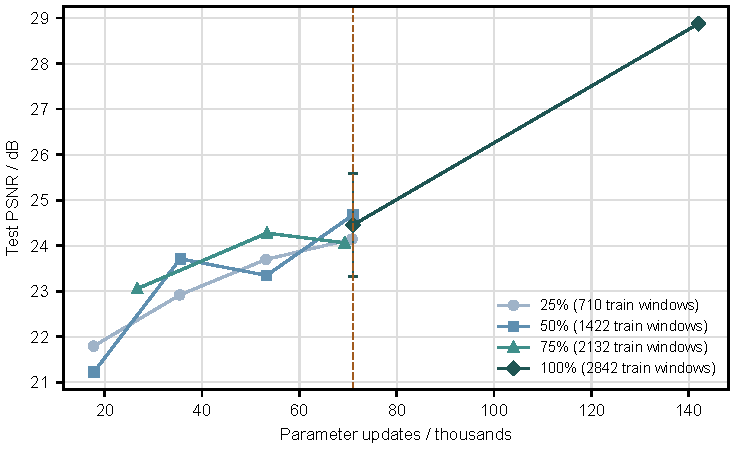
\includegraphics[width=.66\textwidth]{figures/en/results_20261124/budget_curve_en.pdf}
\caption{Test PSNR under matched parameter-update budgets across 25\%, 50\%, 75\%, and 100\% training subsets (4:1 windows).\label{fig:s-budget-curve}}
\end{figure}

\begin{table}[htbp]\centering\small
\caption{Per-site PSNR (dB) under 4:1 random split vs.\ two-fold held-out evaluation.}\label{tab:s-bench-per-scene}
\begin{tabular}{@{}lrrr@{}}
\toprule
Site & Random split & Held-out site & Difference\\
\midrule
C1 & 21.71 & 5.13 & -16.57 \\
C2 & 26.37 & 9.61 & -16.75 \\
C3 & 24.85 & 11.44 & -13.40 \\
C4 & 23.30 & 10.64 & -12.65 \\
C5 & 23.26 & 9.20 & -14.06 \\
C6 & 24.44 & 9.36 & -15.08 \\
C7 & 22.91 & 7.87 & -15.03 \\
C8 & 25.74 & 8.08 & -17.66 \\
C9 & 27.82 & 5.67 & -22.15 \\
C10 & 22.28 & 8.83 & -13.45 \\
\midrule
Ten-site equal mean & 24.27 & 8.58 & -15.68 \\
\bottomrule
\end{tabular}

\end{table}

\begin{figure}[tbp]\centering
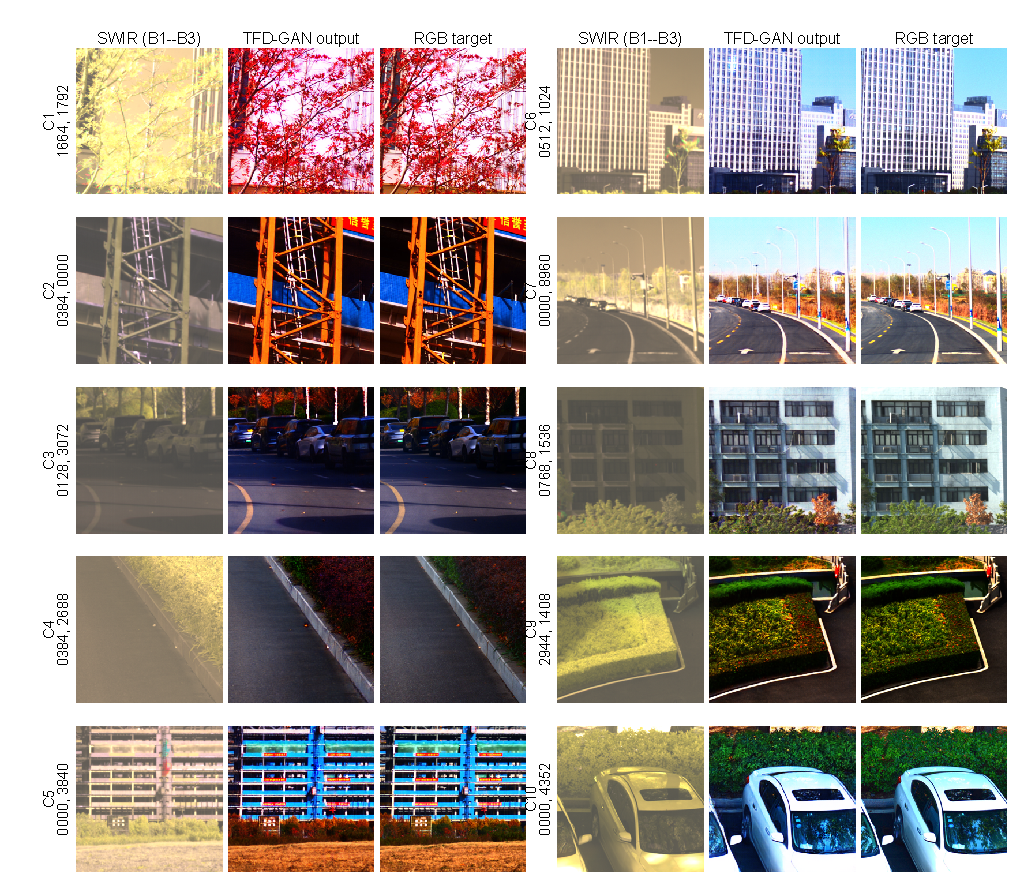
\includegraphics[width=.96\textwidth,height=.74\textheight,keepaspectratio]{figures/en/results_20261124/qualitative_en.pdf}
\caption{Track A (4:1 within-scene random split) TFD-GAN predictions across all ten sites (200 epochs; PSNR \QualPsnrMin--\QualPsnrMax\,dB).\label{fig:s-qualitative}}
\end{figure}

\clearpage
\section*{Supplementary Section 3: Track B Fold Protocol, All 45 Fixed Inputs, Support Statistics, and Validation Curves}

\begin{table}[htbp]\centering\small
\caption{Site-disjoint five-fold assignment.}\label{tab:s-protocol}
\begin{tabular}{@{}clll@{}}\toprule
Fold & Training sites (6) & Validation sites (2) & Test sites (2)\\\midrule
1 & C3,C4,C5,C6,C7,C10 & C2,C9 & C1,C8\\
2 & C1,C3,C4,C6,C7,C8 & C5,C10 & C2,C9\\
3 & C1,C2,C4,C7,C8,C9 & C3,C6 & C5,C10\\
4 & C1,C2,C5,C8,C9,C10 & C4,C7 & C3,C6\\
5 & C2,C3,C5,C6,C9,C10 & C1,C8 & C4,C7\\\bottomrule
\end{tabular}\end{table}

\begin{figure}[htbp]\centering
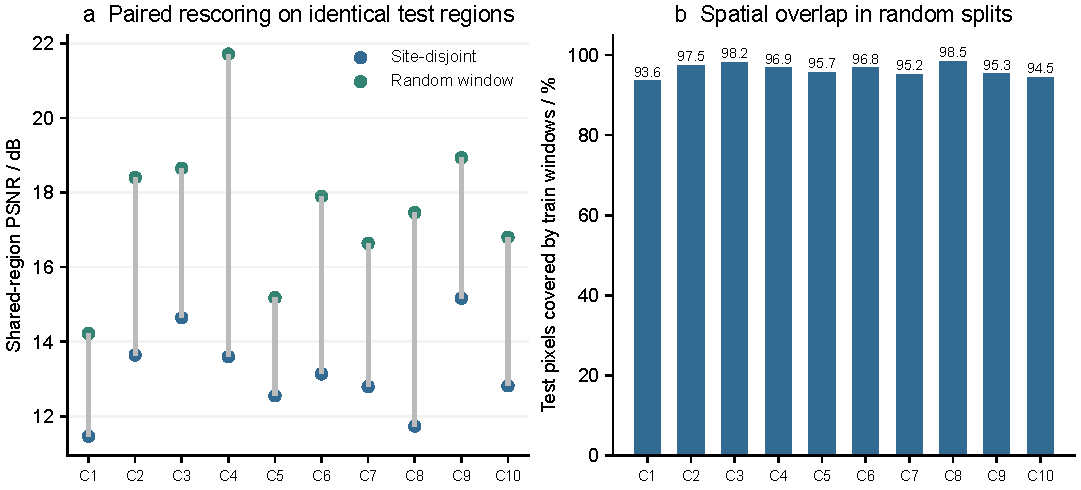
\includegraphics[width=\textwidth,height=.44\textheight,keepaspectratio]{figures/en/results_20261109/protocol_sensitivity.pdf}
\caption{Protocol sensitivity on identical $256\times256$ stride-128 windows (pix2pix, 45 random-split runs vs.\ site-disjoint evaluation; mean inflation +\ProtocolGain\,dB).\label{fig:s-protocol-sensitivity}}
\end{figure}

\begin{table}[htbp]\centering\small
\caption{Validation-selected single-band and three-band inputs per fold.}\label{tab:s-choices}
\begin{tabular}{@{}ccccccc@{}}
\toprule
Fold & DRUNet-1 & DRUNet-3 & pix2pix-1 & pix2pix-3 & TFD-1 & TFD-3\\
\midrule
1 & S3 & T234 & S1 & T135 & S3 & T134\\
2 & S3 & T135 & S2 & T125 & S1 & T125\\
3 & S3 & T134 & S4 & T145 & S3 & T124\\
4 & S3 & T245 & S1 & T124 & S1 & T234\\
5 & S1 & T125 & S4 & T145 & S2 & T134\\
\bottomrule
\end{tabular}

\end{table}

\begingroup\small
\begin{longtable}{@{}llrrrrr@{}}
\caption{Ten-site equal means for all 45 fixed-input conditions (site-disjoint five-fold benchmark). PSNR is in dB.}\label{tab:all-inputs-en}\\
\toprule Model & Input & PSNR↑ & SSIM↑ & LPIPS↓ & \dE{}↓ & MAE↓\\\midrule
\endfirsthead
\multicolumn{7}{r}{\small Continued \thetable}\\
\toprule Model & Input & PSNR↑ & SSIM↑ & LPIPS↓ & \dE{}↓ & MAE↓\\\midrule
\endhead
\midrule\multicolumn{7}{r}{Continued on next page}\\\endfoot\bottomrule\endlastfoot
DRUNet & S1 & 13.610 & 0.578 & 0.667 & 22.102 & 0.162\\
DRUNet & S2 & 13.289 & 0.553 & 0.694 & 24.224 & 0.173\\
DRUNet & S3 & 13.629 & 0.570 & 0.688 & 22.531 & 0.164\\
DRUNet & S4 & 13.369 & 0.566 & 0.698 & 23.882 & 0.169\\
DRUNet & S5 & 13.566 & 0.568 & 0.689 & 22.569 & 0.166\\
DRUNet & T123 & 13.365 & 0.543 & 0.582 & 21.934 & 0.167\\
DRUNet & T124 & 13.347 & 0.561 & 0.621 & 23.391 & 0.163\\
DRUNet & T125 & 13.694 & 0.550 & 0.540 & 20.675 & 0.164\\
DRUNet & T134 & 13.880 & 0.554 & 0.539 & 20.249 & 0.158\\
DRUNet & T135 & 13.595 & 0.567 & 0.529 & 20.843 & 0.161\\
DRUNet & T145 & 13.588 & 0.555 & 0.590 & 21.961 & 0.164\\
DRUNet & T234 & 13.745 & 0.560 & 0.556 & 20.593 & 0.159\\
DRUNet & T235 & 13.688 & 0.545 & 0.555 & 20.952 & 0.165\\
DRUNet & T245 & 14.058 & 0.550 & 0.524 & 20.233 & 0.161\\
DRUNet & T345 & 13.519 & 0.548 & 0.579 & 21.159 & 0.166\\
pix2pix & S1 & 13.240 & 0.470 & 0.608 & 23.662 & 0.165\\
pix2pix & S2 & 12.816 & 0.471 & 0.595 & 24.733 & 0.174\\
pix2pix & S3 & 12.819 & 0.461 & 0.619 & 25.443 & 0.178\\
pix2pix & S4 & 12.663 & 0.476 & 0.594 & 24.316 & 0.178\\
pix2pix & S5 & 12.751 & 0.437 & 0.640 & 25.956 & 0.176\\
pix2pix & T123 & 12.840 & 0.452 & 0.581 & 22.546 & 0.179\\
pix2pix & T124 & 13.118 & 0.452 & 0.580 & 23.066 & 0.168\\
pix2pix & T125 & 12.929 & 0.450 & 0.576 & 23.214 & 0.176\\
pix2pix & T134 & 13.054 & 0.464 & 0.571 & 21.609 & 0.171\\
pix2pix & T135 & 13.141 & 0.436 & 0.593 & 22.687 & 0.170\\
pix2pix & T145 & 12.965 & 0.438 & 0.587 & 22.812 & 0.172\\
pix2pix & T234 & 12.929 & 0.419 & 0.656 & 22.587 & 0.175\\
pix2pix & T235 & 12.838 & 0.438 & 0.575 & 22.976 & 0.174\\
pix2pix & T245 & 12.901 & 0.394 & 0.599 & 21.918 & 0.174\\
pix2pix & T345 & 12.959 & 0.425 & 0.587 & 22.136 & 0.170\\
TFD-GAN & S1 & 11.843 & 0.417 & 0.583 & 25.956 & 0.206\\
TFD-GAN & S2 & 11.997 & 0.423 & 0.591 & 26.899 & 0.199\\
TFD-GAN & S3 & 12.376 & 0.416 & 0.562 & 26.864 & 0.189\\
TFD-GAN & S4 & 12.148 & 0.427 & 0.571 & 25.236 & 0.192\\
TFD-GAN & S5 & 12.569 & 0.421 & 0.569 & 25.896 & 0.184\\
TFD-GAN & T123 & 12.602 & 0.444 & 0.532 & 24.226 & 0.180\\
TFD-GAN & T124 & 12.887 & 0.438 & 0.530 & 23.183 & 0.173\\
TFD-GAN & T125 & 12.555 & 0.423 & 0.543 & 24.622 & 0.185\\
TFD-GAN & T134 & 12.879 & 0.448 & 0.531 & 23.084 & 0.176\\
TFD-GAN & T135 & 12.700 & 0.426 & 0.517 & 24.192 & 0.183\\
TFD-GAN & T145 & 12.760 & 0.407 & 0.564 & 24.469 & 0.182\\
TFD-GAN & T234 & 12.594 & 0.395 & 0.558 & 23.414 & 0.186\\
TFD-GAN & T235 & 12.420 & 0.407 & 0.564 & 24.755 & 0.190\\
TFD-GAN & T245 & 12.339 & 0.424 & 0.529 & 25.447 & 0.190\\
TFD-GAN & T345 & 12.576 & 0.411 & 0.560 & 24.417 & 0.186\\
\end{longtable}

\endgroup

\begin{table}[htbp]\centering\footnotesize
\caption{Per-site evaluation support in Track B (LPIPS coverage uses common valid pixels as denominator).}\label{tab:s-support}
% Generated by make_support_statistics_20261015.py; counts use saved support.
\begin{tabular*}{\textwidth}{@{\extracolsep{\fill}}lrrrrrrr@{}}
\toprule
Site & \shortstack{Common\\Mpx} & \shortstack{Canvas\\(\%)} & \shortstack{SSIM centres\\million} & Windows & \shortstack{LPIPS\\rectangles} & \shortstack{Unique area\\Mpx} & \shortstack{Area/common\\(\%)} \\
\midrule
C1 & 10.653 & 48.97 & 5.153 & 754 & 10 & 0.164 & 1.54 \\
C2 & 13.189 & 77.49 & 7.243 & 936 & 67 & 0.991 & 7.52 \\
C3 & 6.224 & 91.87 & 4.909 & 396 & 214 & 3.257 & 52.34 \\
C4 & 5.837 & 94.02 & 5.406 & 339 & 275 & 4.355 & 74.62 \\
C5 & 9.463 & 71.67 & 5.379 & 678 & 17 & 0.279 & 2.94 \\
C6 & 4.650 & 56.33 & 3.675 & 303 & 88 & 1.435 & 30.85 \\
C7 & 10.479 & 61.05 & 6.730 & 697 & 32 & 0.520 & 4.96 \\
C8 & 12.361 & 64.08 & 12.006 & 770 & 670 & 10.228 & 82.74 \\
C9 & 7.775 & 61.99 & 4.116 & 494 & 135 & 2.108 & 27.11 \\
C10 & 8.231 & 71.44 & 3.915 & 526 & 33 & 0.469 & 5.70 \\
\midrule
Total & 88.861 & 66.45 & 58.532 & 5893 & 1541 & 23.806 & 26.79 \\
\bottomrule
\end{tabular*}

\end{table}

\begin{table}[htbp]\centering\footnotesize
\caption{Per-site and per-modality percentages at $\mathrm{DN}=0$ and $\mathrm{DN}\ge 250$.}\label{tab:s-dynamic}
% Each cell = percent zero / percent >= 250, denominator geometry/privacy pixels.
\begin{tabular*}{\textwidth}{@{\extracolsep{\fill}}lrrrrrr@{}}
\toprule
Site & RGB & B1 & B2 & B3 & B4 & B5 \\
\midrule
C1 & 3.35/40.72 & 0.00/16.23 & 0.00/8.38 & 0.00/0.23 & 0.00/2.55 & 0.00/0.12 \\
C2 & 13.44/9.44 & 0.00/0.10 & 0.00/0.05 & 0.00/0.06 & 0.00/0.04 & 0.00/0.05 \\
C3 & 5.53/2.49 & 0.00/0.72 & 0.00/0.19 & 0.00/0.01 & 0.00/0.01 & 0.00/0.01 \\
C4 & 1.13/1.75 & 0.00/3.52 & 0.00/0.38 & 0.00/0.00 & 0.00/0.00 & 0.00/0.00 \\
C5 & 3.10/14.48 & 0.00/17.01 & 0.00/0.19 & 0.00/0.03 & 0.00/0.02 & 0.00/0.02 \\
C6 & 0.68/41.08 & 0.00/6.72 & 0.00/2.42 & 0.00/0.00 & 0.00/0.03 & 0.00/0.00 \\
C7 & 0.90/31.79 & 0.00/10.10 & 0.00/2.64 & 0.00/0.05 & 0.00/0.18 & 0.00/0.01 \\
C8 & 0.00/35.92 & 0.00/0.00 & 0.00/0.00 & 0.00/0.00 & 0.00/0.00 & 0.00/0.00 \\
C9 & 26.10/11.89 & 0.00/0.04 & 0.00/0.00 & 0.00/0.00 & 0.00/0.00 & 0.00/0.00 \\
C10 & 10.23/15.89 & 0.00/4.75 & 0.00/2.59 & 0.00/1.11 & 0.00/1.65 & 0.00/1.06 \\
\bottomrule
\end{tabular*}

\end{table}

\begin{figure}[htbp]\centering
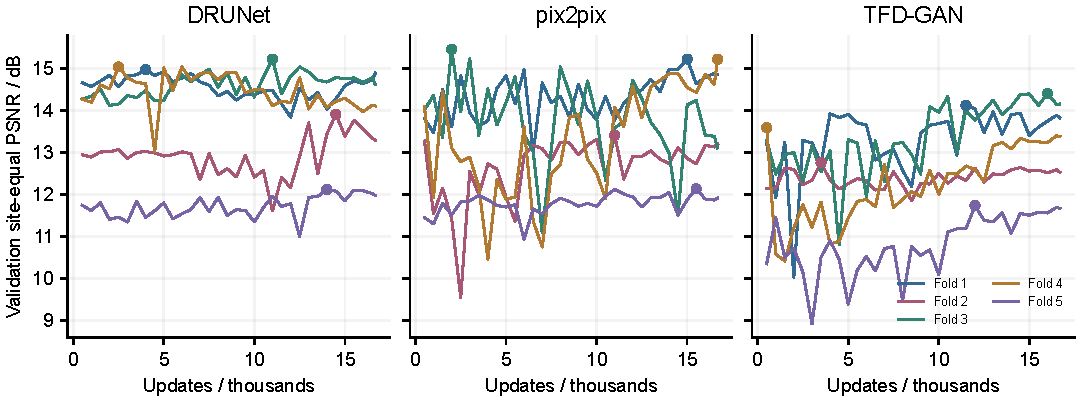
\includegraphics[width=\textwidth,height=.4\textheight,keepaspectratio]{figures/en/results_20261109/validation_curves.pdf}
\caption{Five-fold validation PSNR trajectories for fixed T124 inputs (510 checkpoints across three architectures).\label{fig:s-training-monitor}}
\end{figure}

\clearpage
\section*{Supplementary Section 4: Full 15-Modality-Pair Non-SIFT Geometric Audit and Track C Neural Fine-Tuning}

\begin{table}[htbp]\centering\small
\caption{Independent non-SIFT Sobel-gradient DFT sub-pixel phase-correlation audit across all 15 modality pairs (432 valid $256\times256$ tiles, $10\times$ upsampling, $r_{\mathrm{grad}}\ge 0.25$).}\label{tab:s-geom-15pair}
\begin{tabular}{@{}llrrrrr@{}}
\toprule
Modality pair & Group & Judgeable/\% & Median/px & RMSE/px & P95/px & $\le$2\,px/\%\\
\midrule
RGB--B1 & Cross-modal & 60.0 & 2.34 & 3.89 & 8.03 & 35.1\\
RGB--B2 & Cross-modal & 51.9 & 2.62 & 3.99 & 8.46 & 30.8\\
RGB--B3 & Cross-modal & 45.6 & 2.42 & 3.91 & 7.77 & 40.6\\
RGB--B4 & Cross-modal & 47.5 & 2.44 & 4.02 & 8.14 & 33.7\\
RGB--B5 & Cross-modal & 44.2 & 2.15 & 3.31 & 5.49 & 42.4\\
B1--B2 & Intra-SWIR & 90.7 & 0.28 & 1.46 & 2.07 & 94.4\\
B1--B3 & Intra-SWIR & 78.9 & 0.45 & 1.46 & 2.25 & 94.1\\
B1--B4 & Intra-SWIR & 85.2 & 0.45 & 1.70 & 3.44 & 91.3\\
B1--B5 & Intra-SWIR & 80.6 & 0.70 & 2.33 & 4.59 & 87.1\\
B2--B3 & Intra-SWIR & 79.2 & 0.51 & 1.90 & 2.91 & 90.4\\
B2--B4 & Intra-SWIR & 87.7 & 0.50 & 1.71 & 2.79 & 90.5\\
B2--B5 & Intra-SWIR & 79.4 & 0.72 & 2.02 & 3.19 & 88.3\\
B3--B4 & Intra-SWIR & 80.1 & 0.61 & 1.30 & 2.15 & 93.6\\
B3--B5 & Intra-SWIR & 78.2 & 0.63 & 1.58 & 2.82 & 91.1\\
B4--B5 & Intra-SWIR & 79.9 & 0.45 & 1.64 & 2.19 & 94.2\\
\midrule
\textbf{RGB--SWIR pooled (5 pairs)} & -- & \textbf{49.8} & \textbf{2.37} & \textbf{3.85} & \textbf{7.97} & \textbf{36.2}\\
\textbf{SWIR--SWIR pooled (10 pairs)} & -- & \textbf{82.0} & \textbf{0.51} & \textbf{1.73} & \textbf{2.84} & \textbf{91.5}\\
\bottomrule
\end{tabular}

\end{table}

\begin{figure}[htbp]\centering
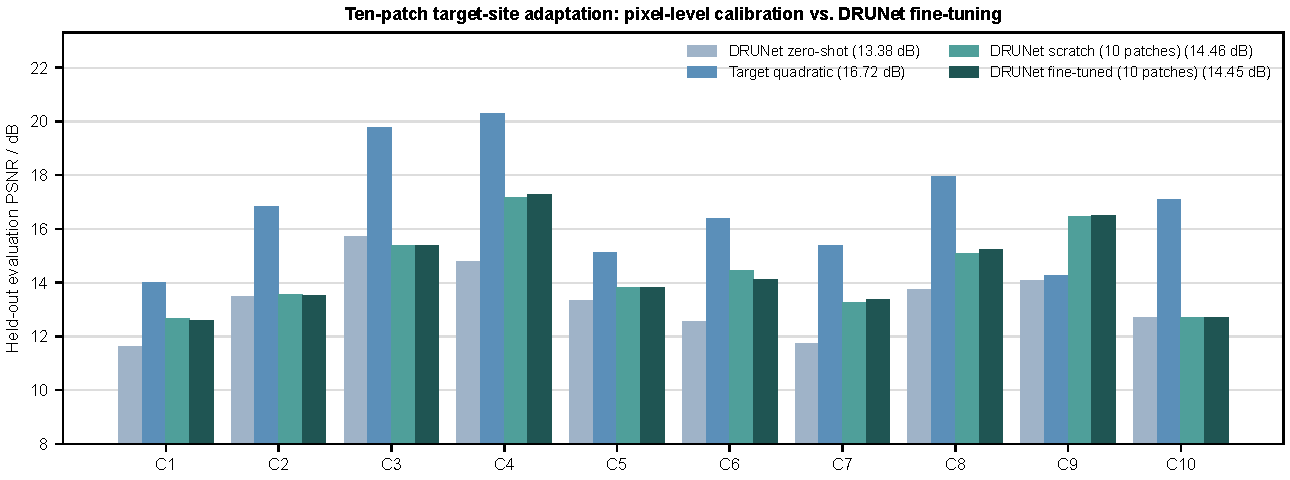
\includegraphics[width=\textwidth]{figures/en/trackc_drunet_en.pdf}
\caption{Per-site Track C comparison on identical 500,000 held-out pixels (fixed B1/B3/B4): DRUNet zero-shot, target-site quadratic calibration, DRUNet scratch (10 patches), and DRUNet fine-tuned (10 patches).\label{fig:s-trackc-drunet}}
\end{figure}

\renewcommand{\bibfont}{\small}
\setlength{\bibsep}{2pt}
\bibliographystyle{unsrtnat}
\bibliography{refs}
\end{document}
